\chapter{Methods}
\label{ch:Methods}

\section{Current Methods}

Here's a table which was generated by \LaTeX. Entering this information manually can be tedious, and prone to error. Use a website like \url{http://www.tablesgenerator.com/} to enter data and automatically generate the \LaTeX code for the table.

\begin{table}[h]
\centering
\caption{Some Data}
\label{tab:data}
\begin{tabular}{|l|c|c|c|c|c|}
\hline
                     &              & \textbf{j=1} & \textbf{j=2} & \textbf{j=3} & \textbf{j=4} \\ \hline
\textbf{Floor-South} & \textbf{i=1} & 0.00000      & 0.00000      & 0.19957      & 0.22824      \\ \hline
\textbf{Floor-North} & \textbf{i=2} & 0.00000      & 0.00000      & 0.05763      & 0.20588      \\ \hline
\textbf{South Wall}  & \textbf{i=3} & 0.19049      & 0.00891      & 0.00000      & 0.22078      \\ \hline
\textbf{East Wall}   & \textbf{i=4} & 0.17429      & 0.02546      & 0.17663      & 0.00000      \\ \hline
\end{tabular}
\end{table}

\section{Better Methods}

\lipsum[1]

\begin{figure}
    \centering
    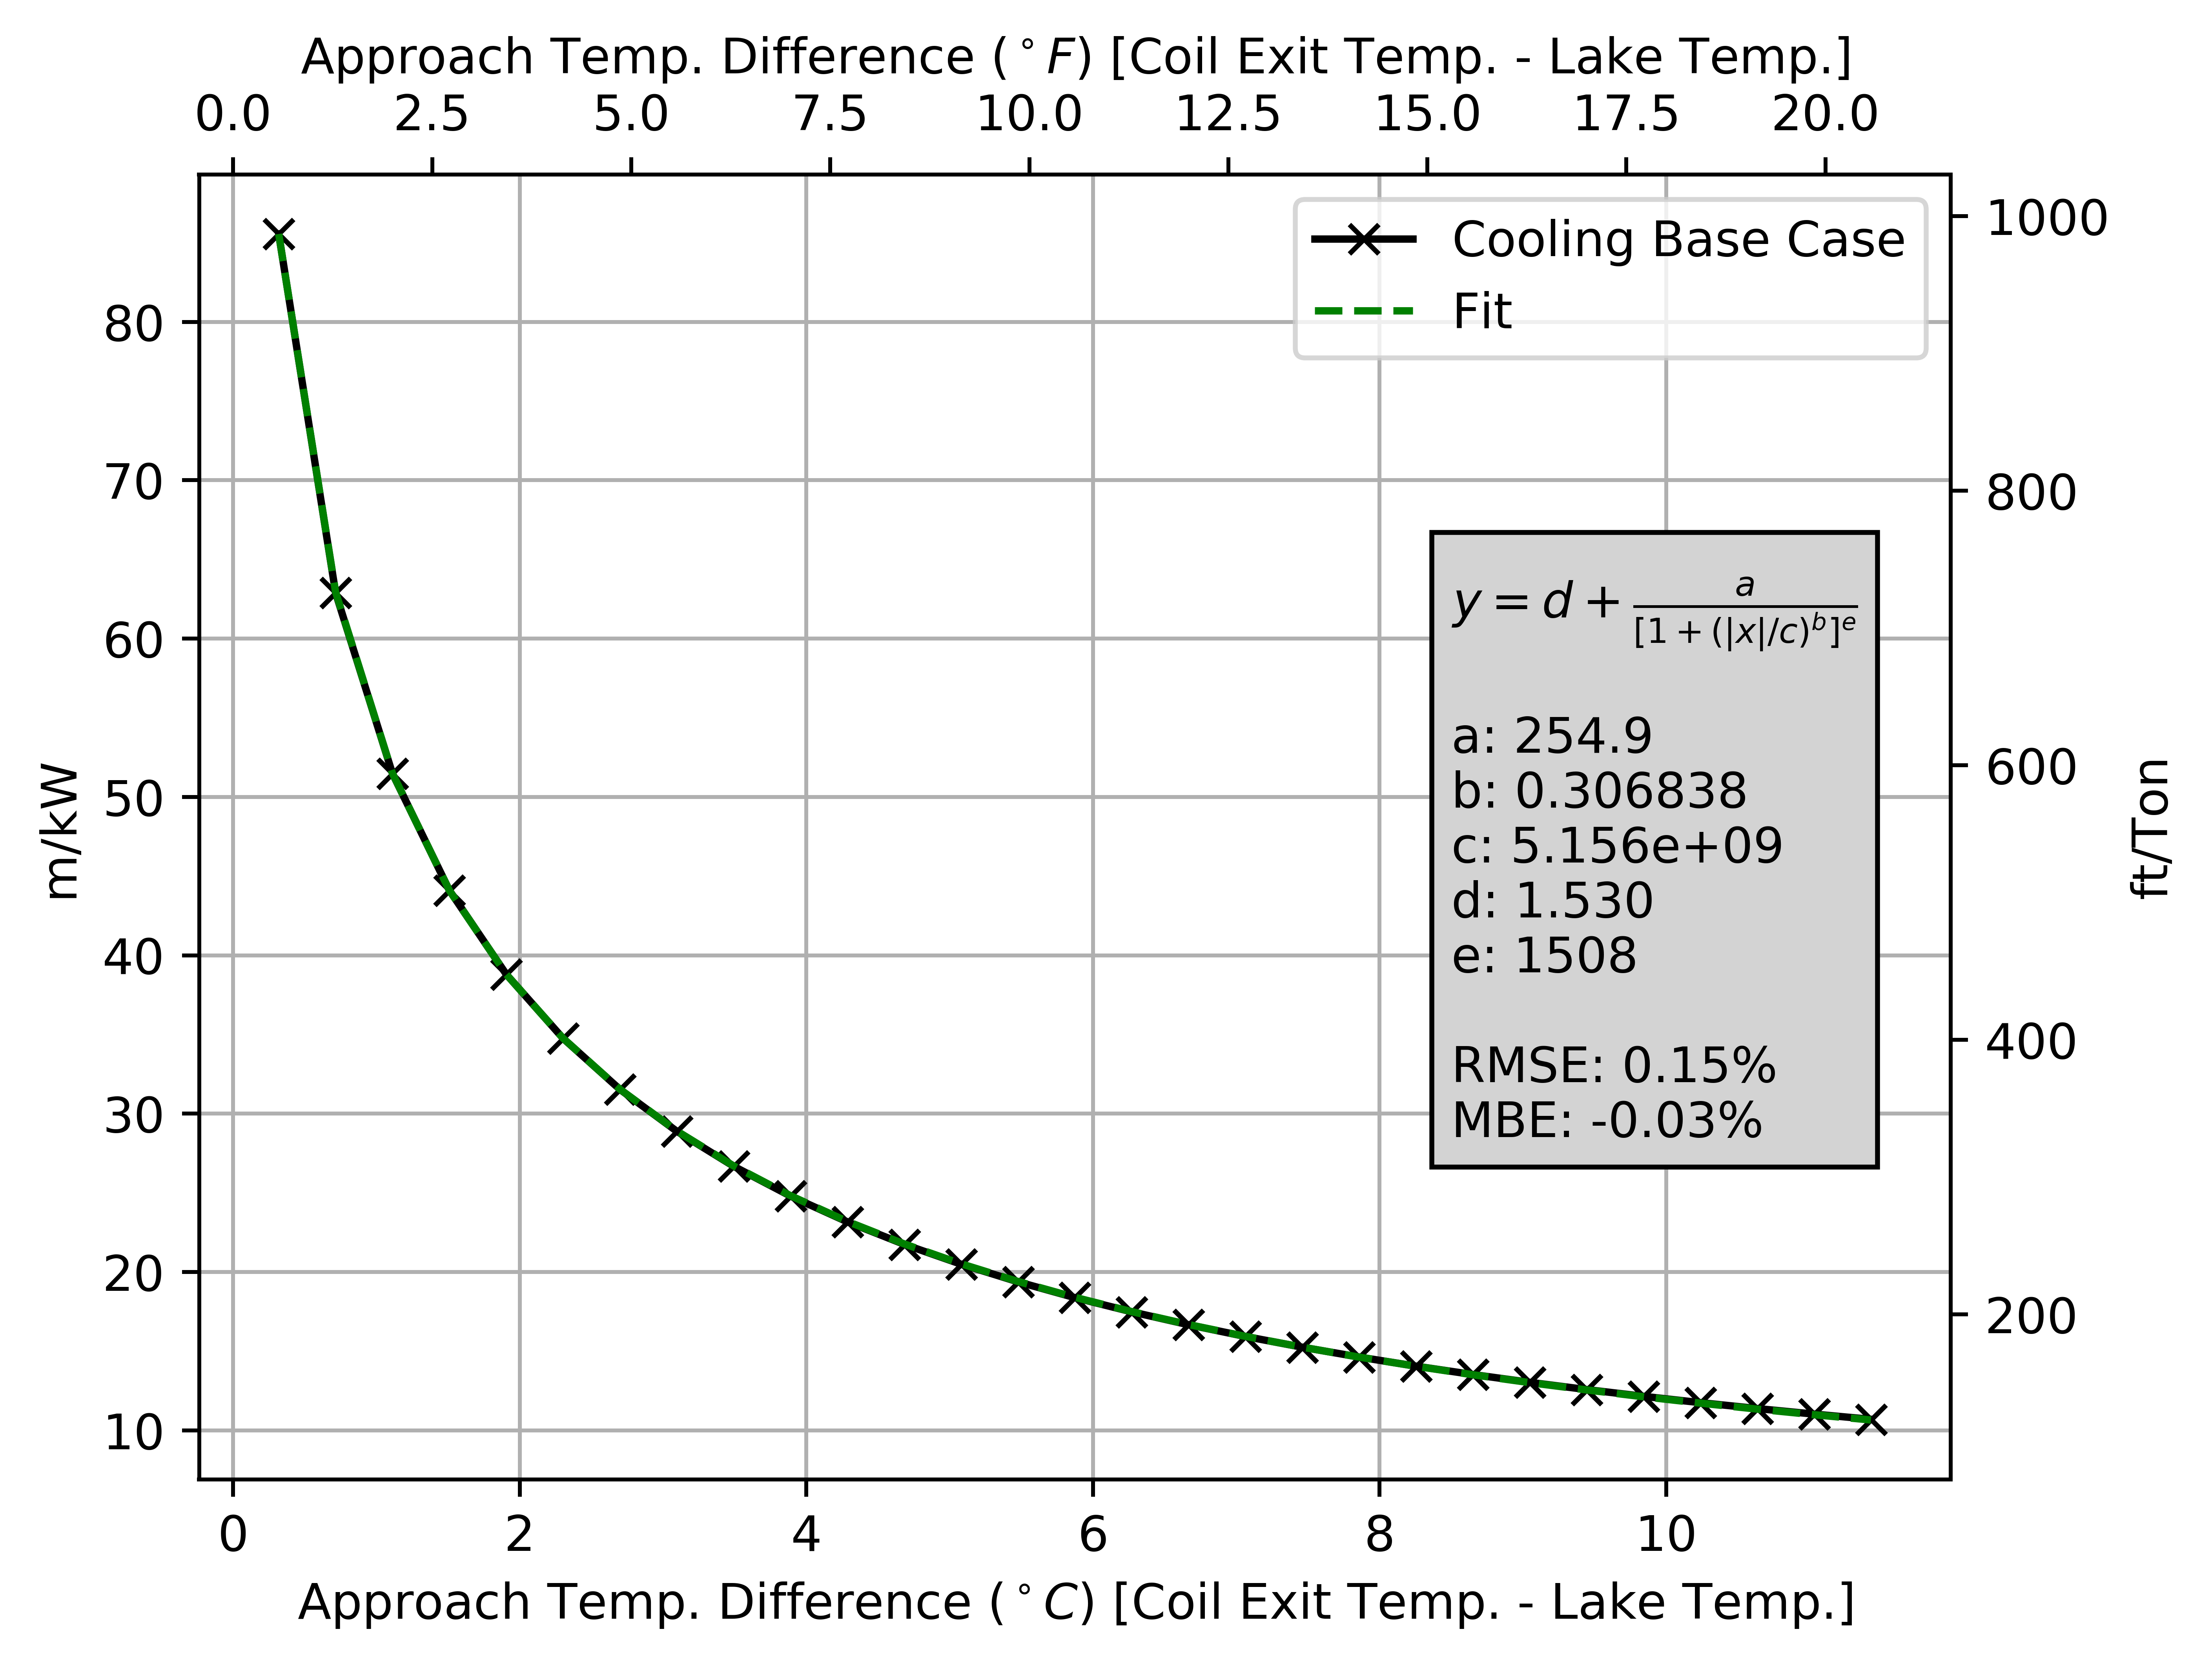
\includegraphics[width=0.75\textwidth]{Cooling_BaseCase_CurveFit.png}
    \caption{Another cool figure}
    \label{fig:another cool figure}
\end{figure}
